\documentclass[conference]{IEEEtran}

% ---------- Packages ----------
\usepackage{newtxtext,newtxmath} % Times系/数式(amssymbは不要)
\usepackage{amsmath}
\usepackage{siunitx}
\usepackage{graphicx,xcolor}
\usepackage{booktabs}
\usepackage{placeins}            % \FloatBarrier
\usepackage[hidelinks]{hyperref}

\usepackage{tikz}
\usetikzlibrary{calc,positioning,fit,arrows.meta,shapes.geometric,shapes.misc}

% ---------- TikZ styles ----------
\tikzset{
  line/.style={-Latex, line width=0.5pt},
  box/.style={draw, rounded corners, align=center, inner sep=3pt},
  smallbox/.style={box, minimum width=28mm, minimum height=7mm},
  midbox/.style={box, minimum width=34mm, minimum height=8mm},
  bigbox/.style={box, minimum width=68mm, minimum height=9mm}
}

%(任意)図まわりの間隔をやや詰める
\setlength{\textfloatsep}{10pt plus 2pt minus 2pt}
\setlength{\floatsep}{8pt plus 2pt minus 2pt}

% ---------- Title ----------
\title{AITL on Space: A Robust Three-Layer Architecture\\
with a Tri-NVM Hierarchy (SRAM / MRAM / FRAM)\\
for Long-Duration Spacecraft Autonomy}

\author{
\IEEEauthorblockN{Shinichi Samizo}
\IEEEauthorblockA{Independent Semiconductor Researcher\\
Former Engineer at Seiko Epson Corporation\\
Email: shin3t72@gmail.com\quad GitHub: \url{https://github.com/Samizo-AITL}}
}

\begin{document}
\maketitle

\begin{abstract}
We propose \emph{AITL on Space}, a robust three-layer control architecture (Robust Core, FSM Supervisor, AI Adaptor) integrated with a tri-NVM hierarchy (SRAM/MRAM/FRAM) and mapped to a 22\,nm FD\!SOI SoC. The contribution is an end-to-end design flow from mission-level specification to ASIC: requirements are formalized as JSON via \texttt{EduController}, synthesized by the \texttt{AITL-H} module, validated in FPGA HIL with fault injection, stress-tested through SystemDK FEM (thermal/radiation/packaging), and finally implemented as ASIC. This methodology enables resilient autonomy for long-duration spacecraft missions.
\end{abstract}

\section{Introduction}
Deep-space missions require ultra-robust control under total ionizing dose (TID), single event effects (SEE), and thermal cycling. Conventional PID\,+\,Flash architectures face lifetime limits due to charge-trap drift and endurance. We present \emph{AITL on Space}: a resilient three-layer architecture with a tri-NVM hierarchy and a reproducible design flow from specification to ASIC.

\section{Specification and Design Flow}
The process begins with \emph{Mission Specification}. Requirements such as pointing accuracy, power stability, and thermal tolerance are captured in \texttt{EduController} (a model-based tool) that exports plant matrices and weighting functions as JSON (portable across simulators). The JSON is consumed by \texttt{AITL-H}, which synthesizes an $H_\infty$ output-feedback controller $K$ with mixed-sensitivity weighting and generates a fixed-point mapping for RTL/FPGA/ASIC. The design then undergoes:
\begin{itemize}
  \item \textbf{FPGA HIL}: hardware-in-the-loop validation with SEU and outage injection; metrics include safe-mode entry \(<\SI{1}{s}\), recovery rate \(\ge\SI{99}{\percent}\), and ECC scrubbing efficiency.
  \item \textbf{SystemDK FEM}: finite-element co-simulation of thermal cycles, radiation effects, and packaging stress, closing the verification loop before silicon.
  \item \textbf{ASIC Mapping}: implementation on GlobalFoundries 22FDX FD\!SOI hardened for long-duration missions.
\end{itemize}

\section{System Architecture}
AITL consists of three layers:
\begin{itemize}
  \item \textbf{Robust Core}: $H_\infty$/MPC/SMC controllers for ultra-robust stability.
  \item \textbf{FSM Supervisor}: mode switching (Safe/Nominal/Recovery) with FDI/FDII for fault management.
  \item \textbf{AI Adaptor}: long-term re-identification and drift compensation.
\end{itemize}
The tri-NVM hierarchy ensures persistence: SRAM for execution, MRAM for logs/code with ECC scrubbing and dual slots, and FRAM for safe boot and FSM states. Target SoC is 22\,nm FD\!SOI hardened against radiation and temperature stress.

\section{Mathematical Model and \texorpdfstring{$H_\infty$}{H-infinity} Design}
We consider an 11D discrete-time state-space plant coupling attitude (6), power bus (2), and thermal nodes (3):
\begin{align}
  x_{k+1} &= A x_k + B u_k + E w_k, \label{eq:ss1}\\
  y_k &= C x_k + D u_k + v_k. \label{eq:ss2}
\end{align}
Here \(w_k\) and \(v_k\) denote disturbance and noise. The model extends to 20D by including translational axes and bias states. Weights \((W_1,W_2,W_3)\) shape sensitivity, control effort, and complementary sensitivity. \texttt{EduController} outputs them as JSON; \texttt{AITL-H} synthesizes \(K\) with robustness margins and exports a fixed-point realization for RTL/FPGA/ASIC.

\section{Verification Pipeline}
FPGA HIL injects SEU bursts and sensor outages. Metrics include safe-mode entry \(<\SI{1}{s}\), recovery \(\ge\SI{99}{\percent}\), and ECC scrubbing efficiency. SystemDK FEM validates thermal and radiation stress, ensuring packaging reliability before ASIC tape-out.

\section{Conclusion}
AITL on Space combines robust control, supervisory safety, AI re-identification, and hardened memory. The proposed end-to-end flow---from mission specification to ASIC---provides a reproducible methodology for resilient autonomy in long-duration space missions.

% ---------- References ----------
\begin{thebibliography}{99}
\bibitem{doyle}
J.\,C.~Doyle, B.\,A.~Francis, and A.\,R.~Tannenbaum,
\emph{Feedback Control Theory}. Macmillan, 1992.

\bibitem{colinge}
J.-P.~Colinge, \emph{Silicon-on-Insulator Technology: Materials to VLSI}, 3rd~ed. Springer, 2004.

\bibitem{wolf}
W.~Wolf, \emph{FPGA-Based System Design}. Prentice Hall, 2004.

\bibitem{rabaey}
J.~M.~Rabaey, A.~Chandrakasan, and B.~Nikoli\'c, \emph{Digital Integrated Circuits: A Design Perspective}, 2nd~ed. Prentice Hall, 2003.
\end{thebibliography}

% ---------- Biography ----------
\section*{Author Biography}
Shinichi Samizo received the M.S.\ degree in Electrical and Electronic Engineering from Shinshu University, Japan. He worked at Seiko Epson Corporation as an engineer in semiconductor memory and mixed-signal device development, and contributed to inkjet MEMS actuators and PrecisionCore printhead technology. He is currently an independent semiconductor researcher focusing on process/device education, memory architecture, and AI system integration. Contact: \texttt{shin3t72@gmail.com}.

% ---------- Flush all floats before figures section ----------
\FloatBarrier

% ---------- Figures (gathered at the end) ----------
\section*{Figures}

% Fig.1: JSON → ASIC flow (2段抜き)
\begin{figure*}[!t]
\centering
\begin{tikzpicture}[node distance=6mm,
  step/.style={box, minimum width=36mm, minimum height=8mm, fill=gray!8}]
  \node[step, fill=purple!10] (spec) {Mission Specification};
  \node[step, fill=blue!10, below=of spec] (json) {EduController JSON Export};
  \node[step, fill=green!12, below=of json] (hinf) {AITL-H $H_\infty$ Synthesis};
  \node[step, fill=orange!18, below=of hinf] (hil) {FPGA HIL Verification};
  \node[step, fill=red!10, below=of hil] (asic) {22FDX ASIC Implementation};
  \node[step, fill=cyan!12, right=20mm of hil] (fem) {\shortstack{SystemDK FEM\\Thermal / Radiation / Packaging}};
  \draw[line] (spec) -- (json);
  \draw[line] (json) -- (hinf);
  \draw[line] (hinf) -- (hil);
  \draw[line] (hil) -- (asic);
  \draw[line] (hil) -- (fem);
\end{tikzpicture}
\caption{End-to-end design flow: Mission Spec \(\rightarrow\) JSON (\texttt{EduController}) \(\rightarrow\) \texttt{AITL-H} \(\rightarrow\) FPGA HIL \(\rightarrow\) SystemDK FEM \(\rightarrow\) ASIC.}
\label{fig:flow}
\end{figure*}

% Fig.2: Architecture (直交配線・斜め矢印なし)
\begin{figure}[!t]
\centering
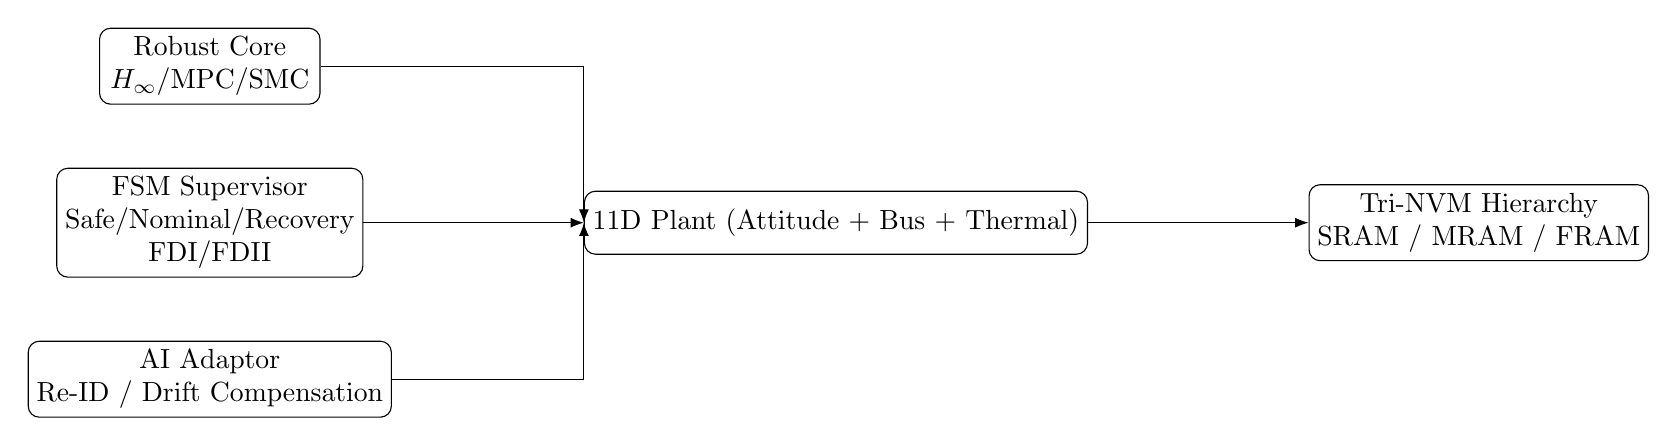
\begin{tikzpicture}[node distance=4mm,>=Latex,
  box/.style={draw,rounded corners,align=center,inner sep=3pt,minimum height=8mm}]
  \node[box,minimum width=28mm] (core) {Robust Core\\$H_\infty$/MPC/SMC};
  \node[box,below=8mm of core,minimum width=28mm] (fsm) {FSM Supervisor\\Safe/Nominal/Recovery\\FDI/FDII};
  \node[box,below=8mm of fsm,minimum width=28mm] (ai)  {AI Adaptor\\Re-ID / Drift Compensation};
  \node[box,right=28mm of fsm,minimum width=55mm] (plant) {11D Plant (Attitude + Bus + Thermal)};
  \node[box,right=28mm of plant,minimum width=36mm] (nvm) {Tri-NVM Hierarchy\\SRAM / MRAM / FRAM};
  % orthogonal interconnects
  \draw[->] (core.east) -| ([yshift=0pt]plant.west);
  \draw[->] (fsm.east) -- (plant.west);
  \draw[->] (ai.east)  -| ([yshift=0pt]plant.west);
  \draw[->] (plant.east) -- (nvm.west);
\end{tikzpicture}
\caption{AITL architecture: three control layers with tri-NVM memory hierarchy. Orthogonal wiring (no diagonal lines) improves readability.}
\label{fig:arch}
\end{figure}

% Fig.3: Closed-loop block diagram
\begin{figure}[!t]
\centering
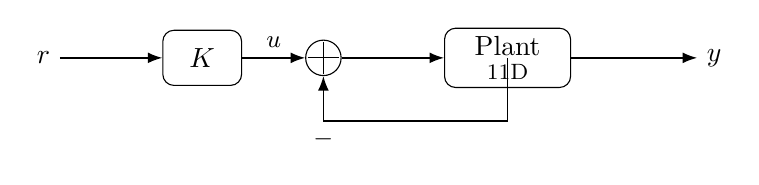
\begin{tikzpicture}[node distance=10mm,>=Latex]
  \node[smallbox, minimum width=10mm] (K) {$K$};
  \node[circle, draw, minimum size=4.5mm, right=8mm of K] (sum) {};
  \draw (sum) +(-2mm,0) -- +(2mm,0);
  \draw (sum) +(0,-2mm) -- +(0,2mm);
  \node[smallbox, right=13mm of sum, minimum width=16mm] (P) {\shortstack{Plant\\\footnotesize 11D}};
  \node[right=16mm of P] (y) {$y$};
  \node[left=13mm of K] (r) {$r$};
  \draw[line] (r) -- (K);
  \draw[line] (K) -- node[above]{\small $u$} (sum);
  \draw[line] (sum) -- (P);
  \draw[line] (P) -- (y);
  \draw[line] ($(P.north)!0.5!(P.south)$) |- ++(0,-8mm) -| node[below]{\small $-$} (sum.south);
\end{tikzpicture}
\caption{Closed-loop system for $H_\infty$ mixed-sensitivity synthesis on the 11D plant.}
\label{fig:loop}
\end{figure}

\end{document}
